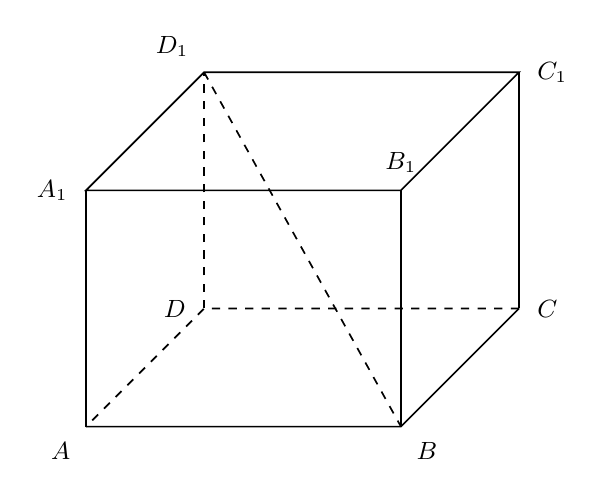
\begin{tikzpicture}[line width=.6pt, font=\small]
\coordinate (A) at (0,0);
\coordinate (B) at (4,0);
\coordinate (C) at (5.5,1.5);
\coordinate (D) at (1.5,1.5);
\coordinate (A1) at (0,3);
\coordinate (B1) at (4,3);
\coordinate (C1) at (5.5,4.5);
\coordinate (D1) at (1.5,4.5);
% bottom face
\draw (A) -- (B) -- (C);
\draw[dashed] (C) -- (D) -- (A);
% top face
\draw (A1) -- (B1) -- (C1) -- (D1) -- cycle;
% verticals
\draw (A) -- (A1);
\draw (B) -- (B1);
\draw (C) -- (C1);
\draw[dashed] (D) -- (D1);
% body diagonal
\draw[dashed] (D1) -- (B);
\node[below left=2pt] at (A) {$A$};
\node[below right=2pt] at (B) {$B$};
\node[right=3pt] at (C) {$C$};
\node[left=3pt] at (D) {$D$};
\node[left=3pt] at (A1) {$A_{1}$};
\node[above=3pt] at (B1) {$B_{1}$};
\node[right=3pt] at (C1) {$C_{1}$};
\node[above left=2pt] at (D1) {$D_{1}$};
\end{tikzpicture}
